\documentclass{article}
\usepackage[utf8]{inputenc}
\usepackage{caption}
\usepackage{amsmath}
\usepackage{amssymb}
\usepackage{mathtools}
\usepackage{multicol}
\usepackage{graphicx}
\usepackage{wrapfig}
\usepackage{float}
\usepackage[makeroom]{cancel}
\usepackage{mhchem}
\usepackage{pst-plot}

\graphicspath{ {../images/} }

\renewcommand{\familydefault}{\sfdefault}
\renewcommand{\baselinestretch}{1.5} % line spacing
\newcommand{\fline}{\par\noindent\rule{\textwidth}{0.1pt}} % horizontal line (wide)

\title{Topic 8 Acids \& Bases\\Lesson 5 - Buffers}
\author{Peter Zhang}

\begin{document}

\maketitle
\tableofcontents
\newpage

% lesson 
\section{Buffers}
They act to reduce the ipmact of acid/base interactions. Without the buffer, extreme changes sometimes occur with minimal volume changes between acid \& base.

\begin{itemize}
\item Buffers do not interefere with Activation Energy
\begin{figure}[H]
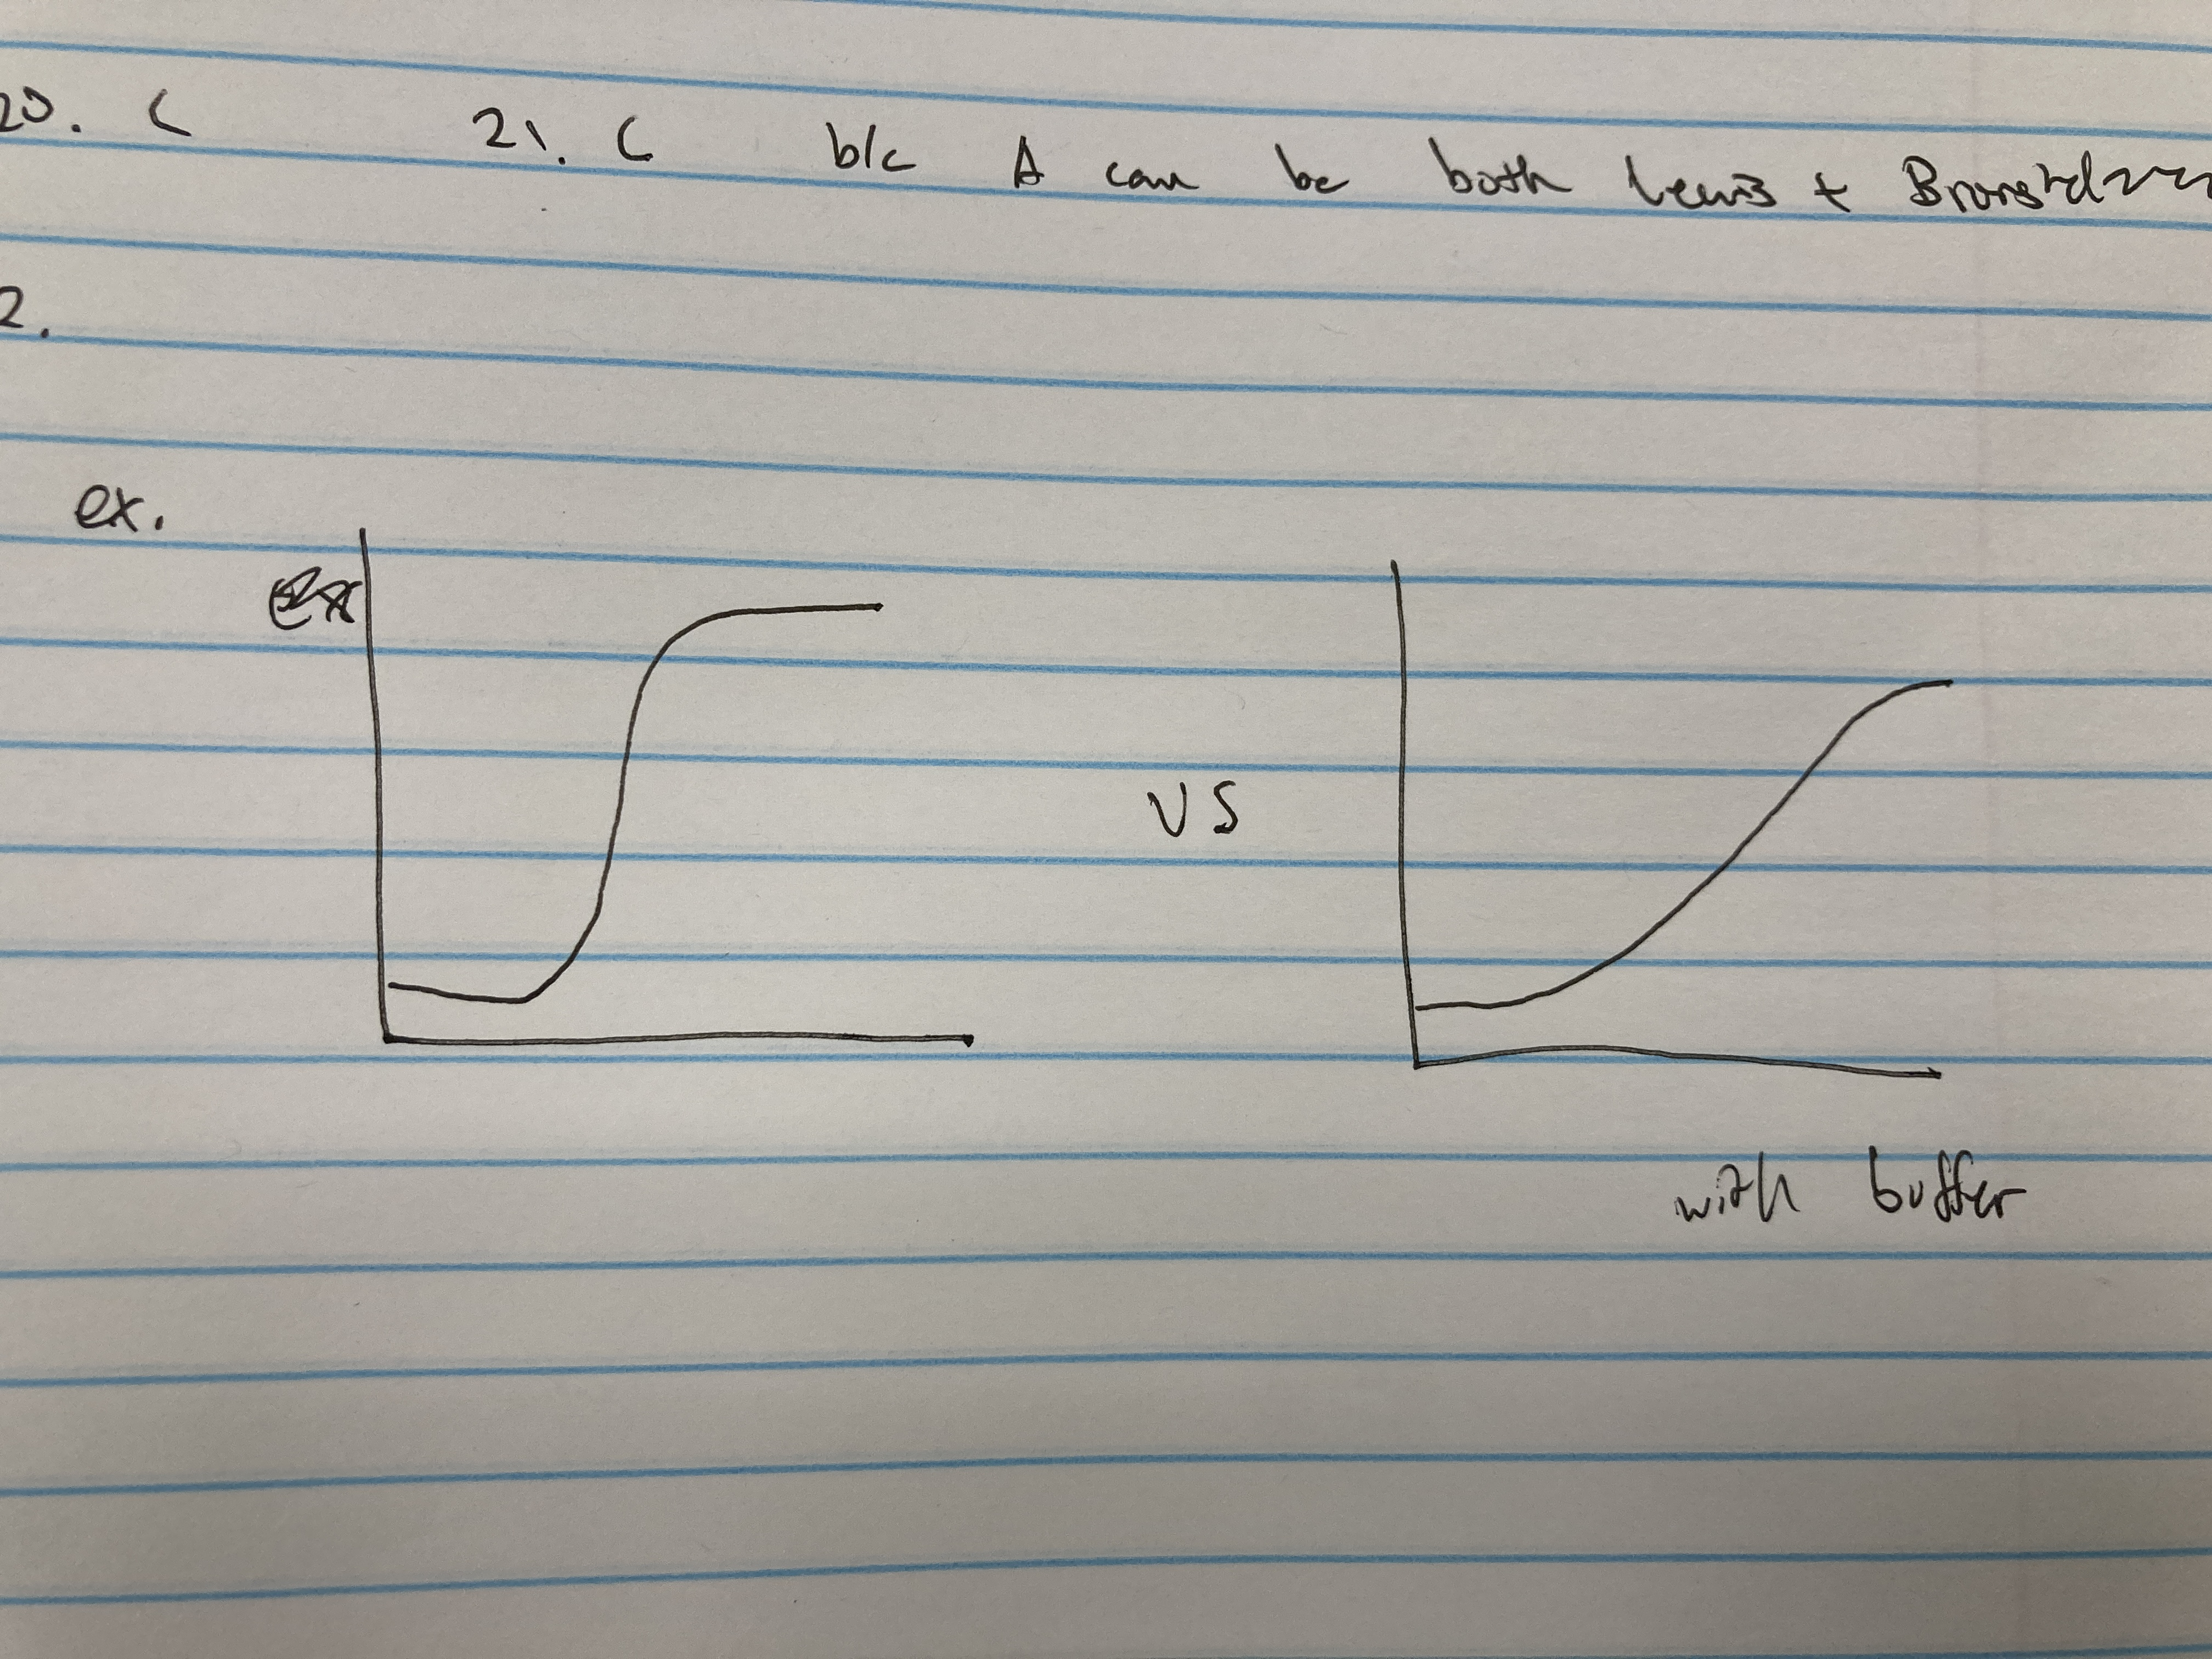
\includegraphics[width=\textwidth]{4.5fig1.jpg}
\captionof{figure}{Example of (rate or smth) with and without a buffer}
\end{figure}
\pagebreak
\subsection{Types of Buffers}
\item There are 2 types of Buffers:
\begin{enumerate}
\item Acidic\\maintains a pH of less than 7. These are usually weak acids with a solution of its salt from a strong aklali (strong alkali = group 1 metal) 
$$\ce{CH3COOH \rightleftharpoons CH3COO- + H+}$$
The left is a weak acid so eequilibrium favors the reactants (left).
$$\ce{NaCH3COO \rightarrow Na+ + CH3COO-}$$
This reaction helps to increase the concentration of the conjugate base.

\textbf{\underline{If an acid is added to this buffer solution}}, the acid should increase the \ce{[H+]} and thus, \textbf{INCREASING IN ACIDIC (or base when needed) PROPERTIES}. The \ce{H+} would combine with \ce{CH3COO-} to form more \ce{CH3COOH}
\begin{itemize}
\item increases the concentration of \ce{CH3COOH}
\item thus, overall reaction rate decreases
\item equilibrium shifts to left (reactants)
\end{itemize}

\textbf{\underline{If a base is added to the buffer solution}}, \ce{OH-} will combine with \ce{CH3COOH} to form \ce{CH3COO-} and \ce{H2O}.  \\\textbf{Reduces impact of most of the \ce{OH-} in the solution.}

% basic buffers
\item Basic\\maintains a pH greater than 7. These are usually a weak base with the salt of a strong acid
$$\ce{NH3 + NH4Cl}$$
$$\ce{NH3 + H2O \rightleftharpoons NH4+ + OH-}$$
$$\ce{NH4Cl(aq) \rightarrow NH4+ + Cl-}$$
reuse causes increase in concentration of conjugate acid\\\\
If an acid is added:
\begin{itemize}
\item \ce{H+} will combine with the \ce{NH3} to form \ce{NH4+}
\item $\therefore $ reduces impact of added \ce{H+}
\end{itemize}
If a base is added:
\begin{itemize}
\item \ce{OH-} with combine with \ce{NH4+} to form \ce{NH4OH} which decomposes to \ce{NH3 + H2O}
\item reduces the impact of the \ce{OH} that are added to the system  
\end{itemize}
\end{enumerate}
\end{itemize}

\subsection{Points}
\begin{enumerate}
% points
\item All buffer systems have a buffering capacity
\item a limit ot when they are unable to resist change
\item \textbf{any dilutions} or temperature changes would also affect pH and the buffering capacity of any buffer being used.
\end{enumerate}

\section{Examples}
\begin{enumerate}
\item A buffer solution is preparid by choosing a weak acid (or base) that has a pKa (or pKb) as close as possible to the required pH.\\ If the pH of an acid is 3.5 and a quick change once the base is added is near a pH of 4, we would look for a weak acid with a pKa close to 4 to make the buffer solution.
\begin{itemize}
\item Buffers should be 1:1 with weak acid (or base) + salt. 
\item 2:1 with weak acid (or base) for the buffer to the acid or base being added $$\ce{CH3COOH + NaOH}$$ If the acid is 2M and the base is 1M.
\end{itemize}
\end{enumerate}




\end{document}